\section{Printed Circuit Board Design}
\subsection{Dimensions}
The \gls{ceenc} is based on the footprint of the \gls{pi}, and as such has stringent design requirements in terms of component layout and dimension.
GPIO headers must be carried across boards, as well as power connections and mounting points. Board length and width must also match that of the \gls{pi}. 

\subsection{Placement}
These requirements dictate the layout of major components, but leave many of the minor pieces unaccounted for.
After allocating areas for the Microcontroller and Power Supply, major connectors are placed for optimal access to the remaining GPIO.
Indicator LED’s, and test points are also placed for ease of use during the testing phase, and components are tweaked to provide an aesthetically pleasing, symmetrical layout.
The Microcontroller is centrally located, to minimize trace lengths to the outlying components.

\subsection{Power Considerations}
Power supply circuitry is isolated to a single section of the board, so as to limit the potential for interference.
Smoothing capacitors are placed as close as possible to the components for which they will be acting, and indicator LED’s are used to mark active lines.
Larger trace widths are used for power lines as a rule of thumb, but of special consideration are the 10 Amp (instantaneous) lines to feed the driver board.
Positive and zero rails are also routed alongside one another, so as to counteract RF interferences that would otherwise result from the voltage differences.

\begin{figure}[h]
	\centering
	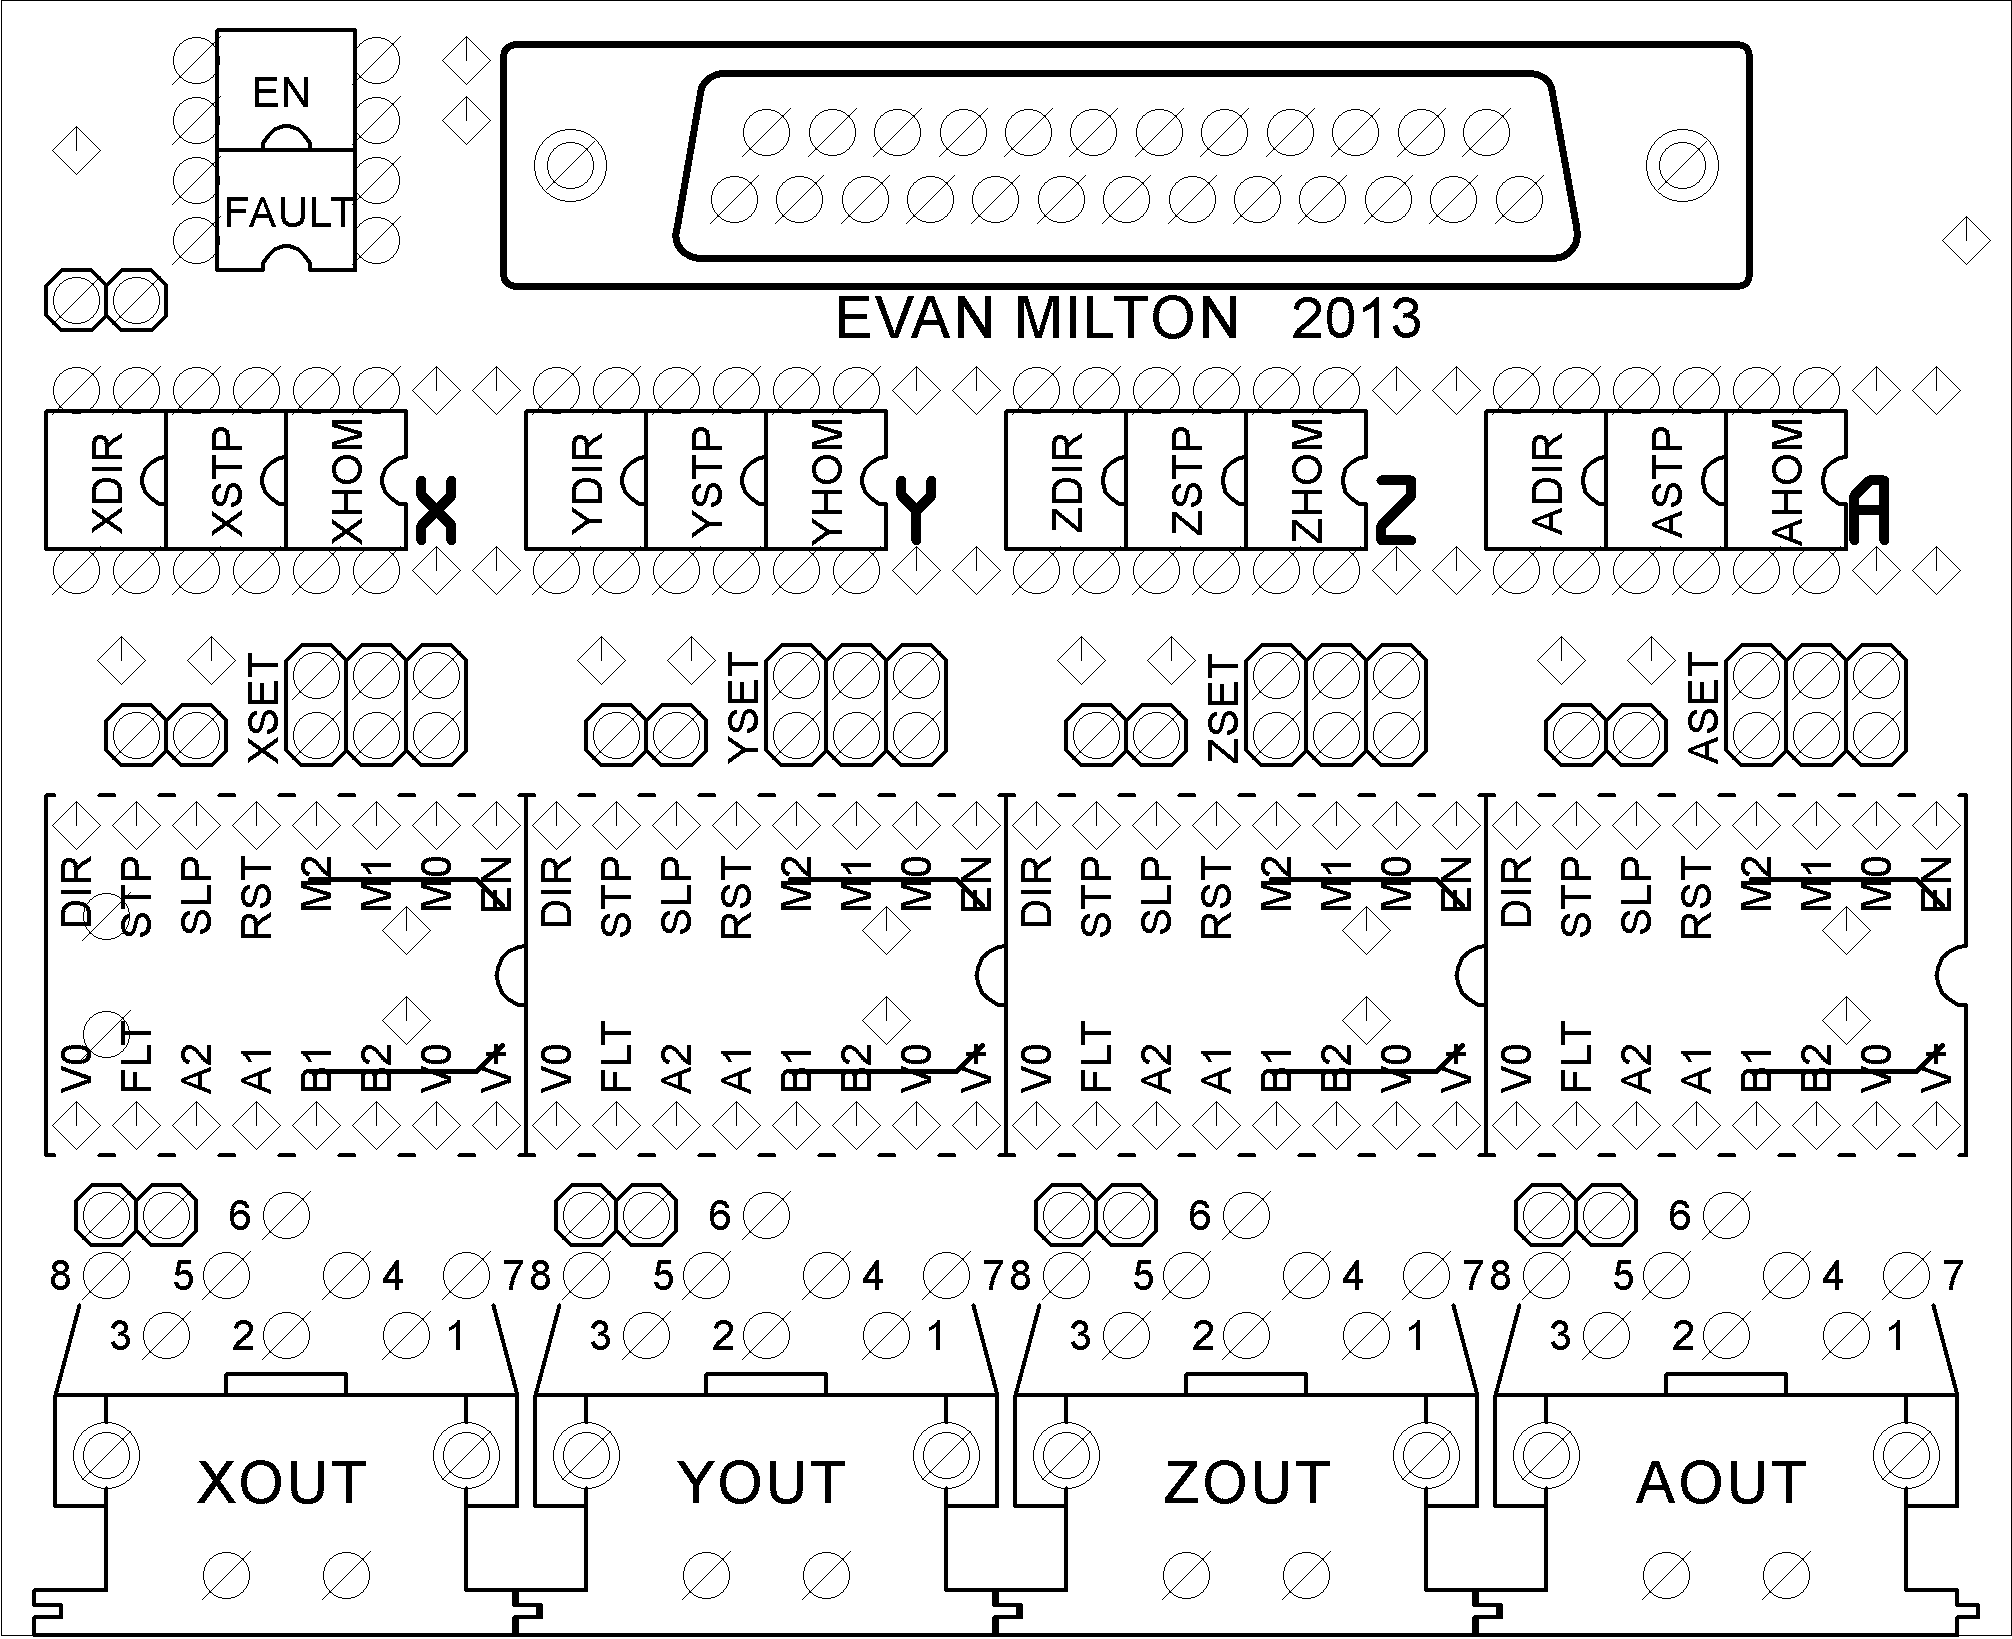
\includegraphics[width=1\textwidth]{pcb-design/topcream.png}
	\caption{Top Cream Layer}
	\label{fig:front}
\end{figure}
\begin{figure}[h]
	\centering
	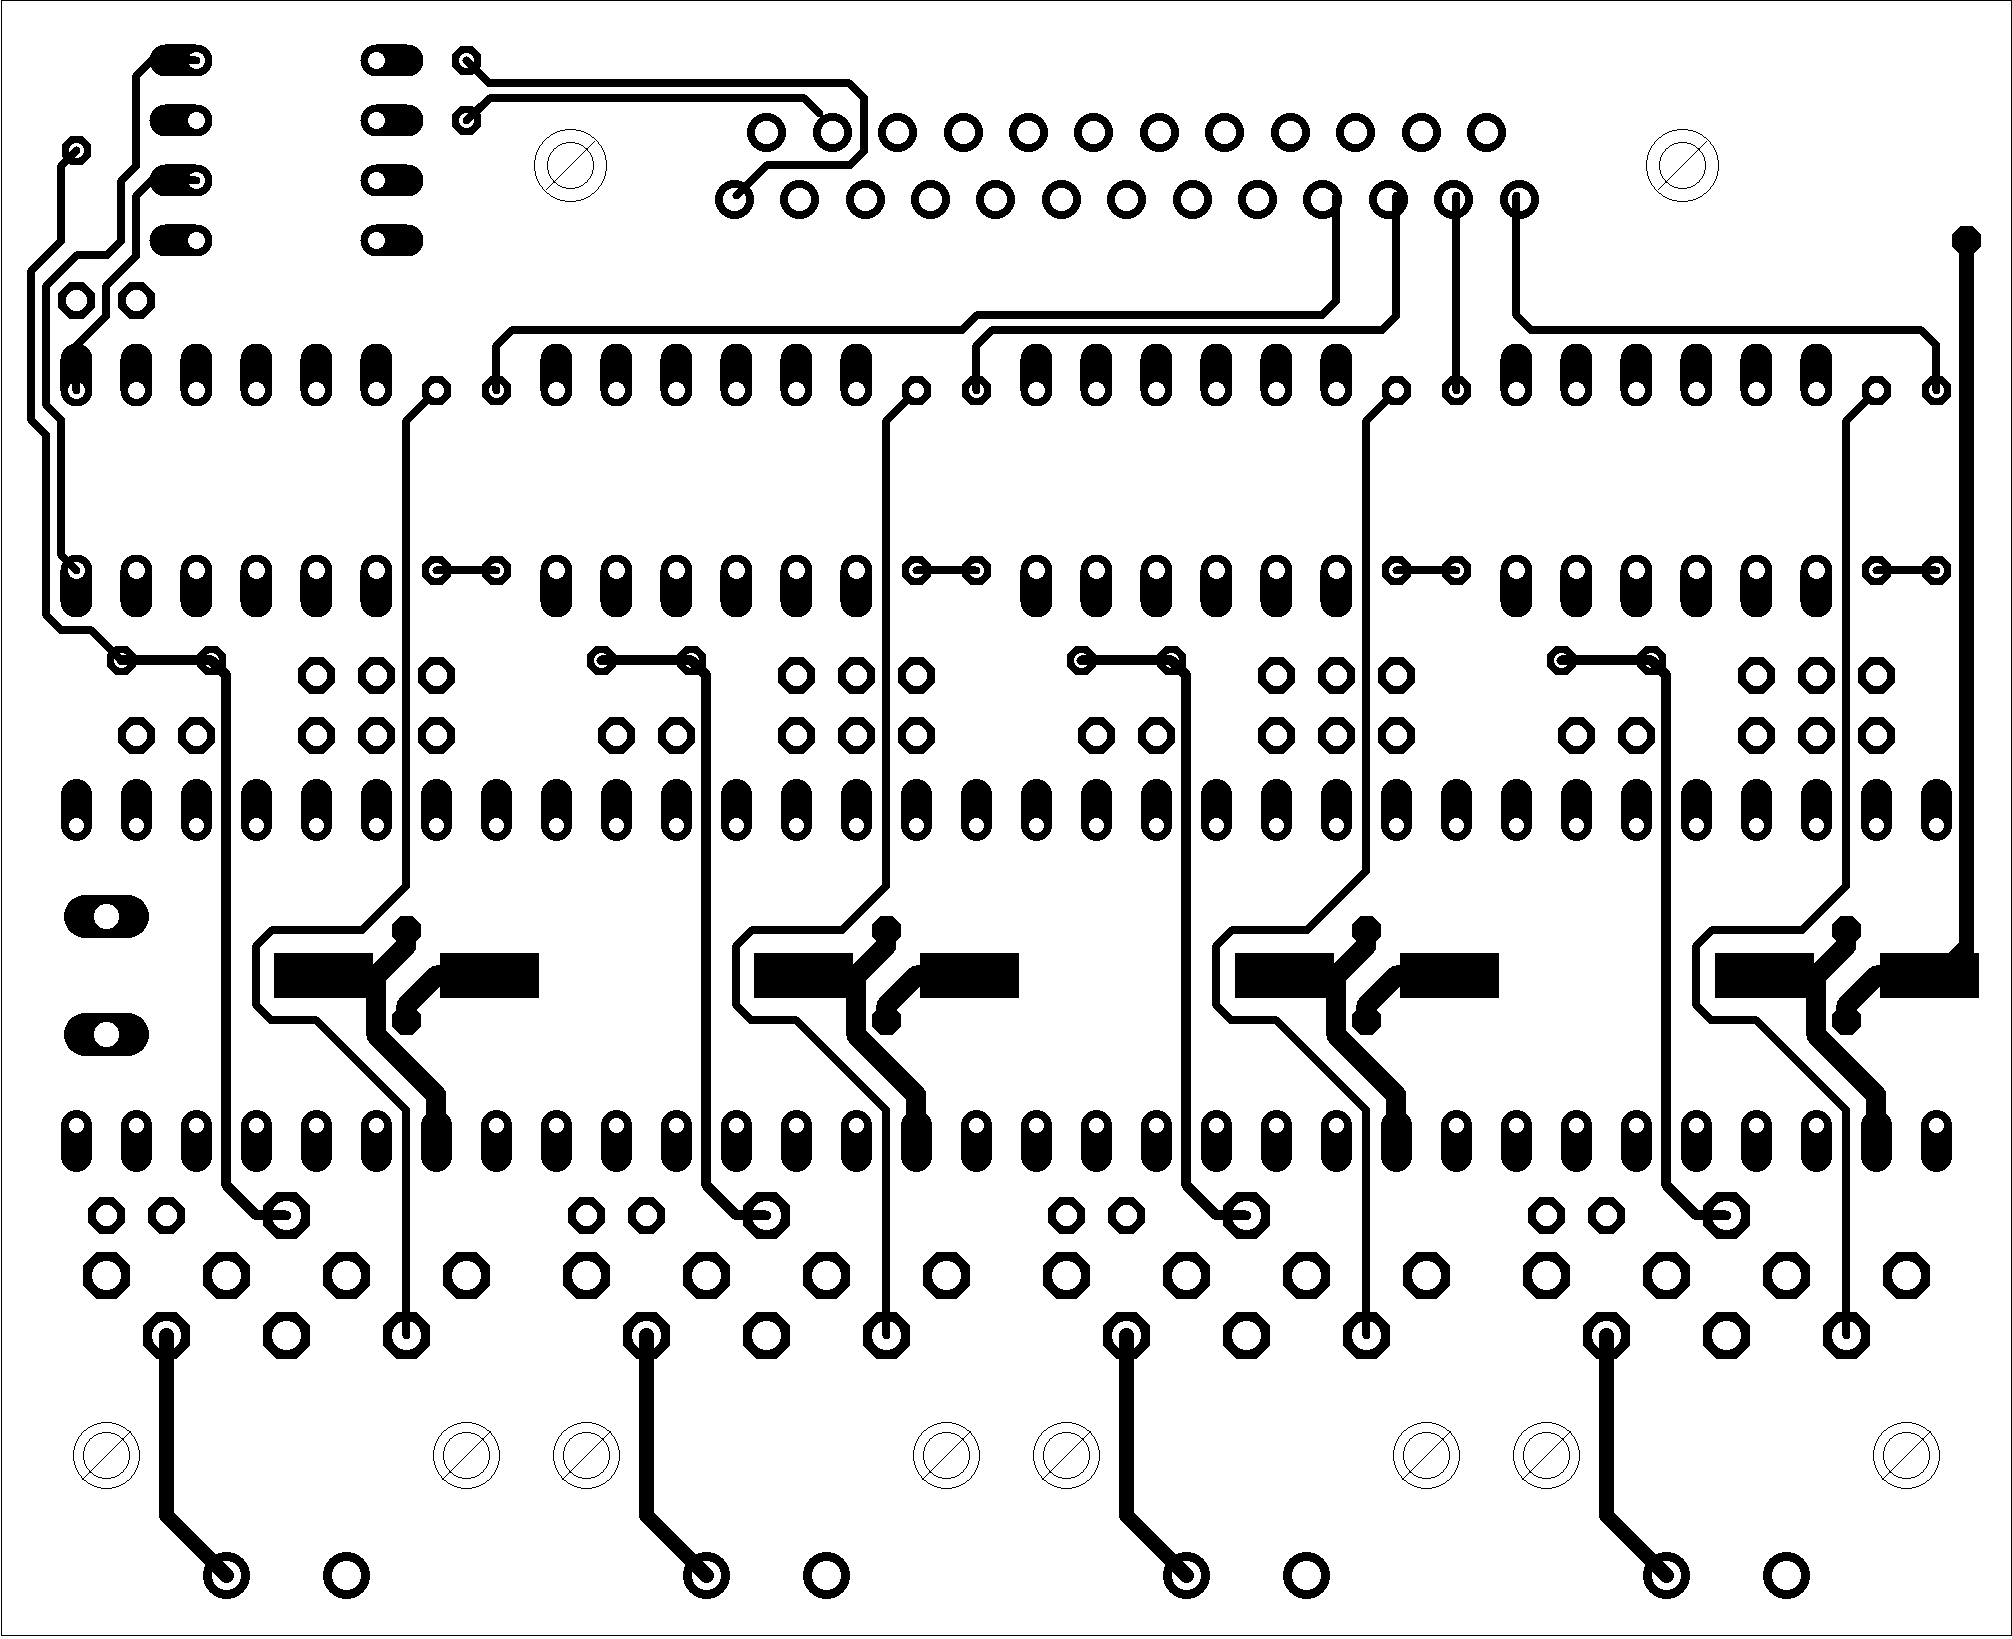
\includegraphics[width=1\textwidth]{pcb-design/toproute.png}
	\caption{Top Copper Layer}
	\label{fig:front}
\end{figure}
\begin{figure}[h]
	\centering
	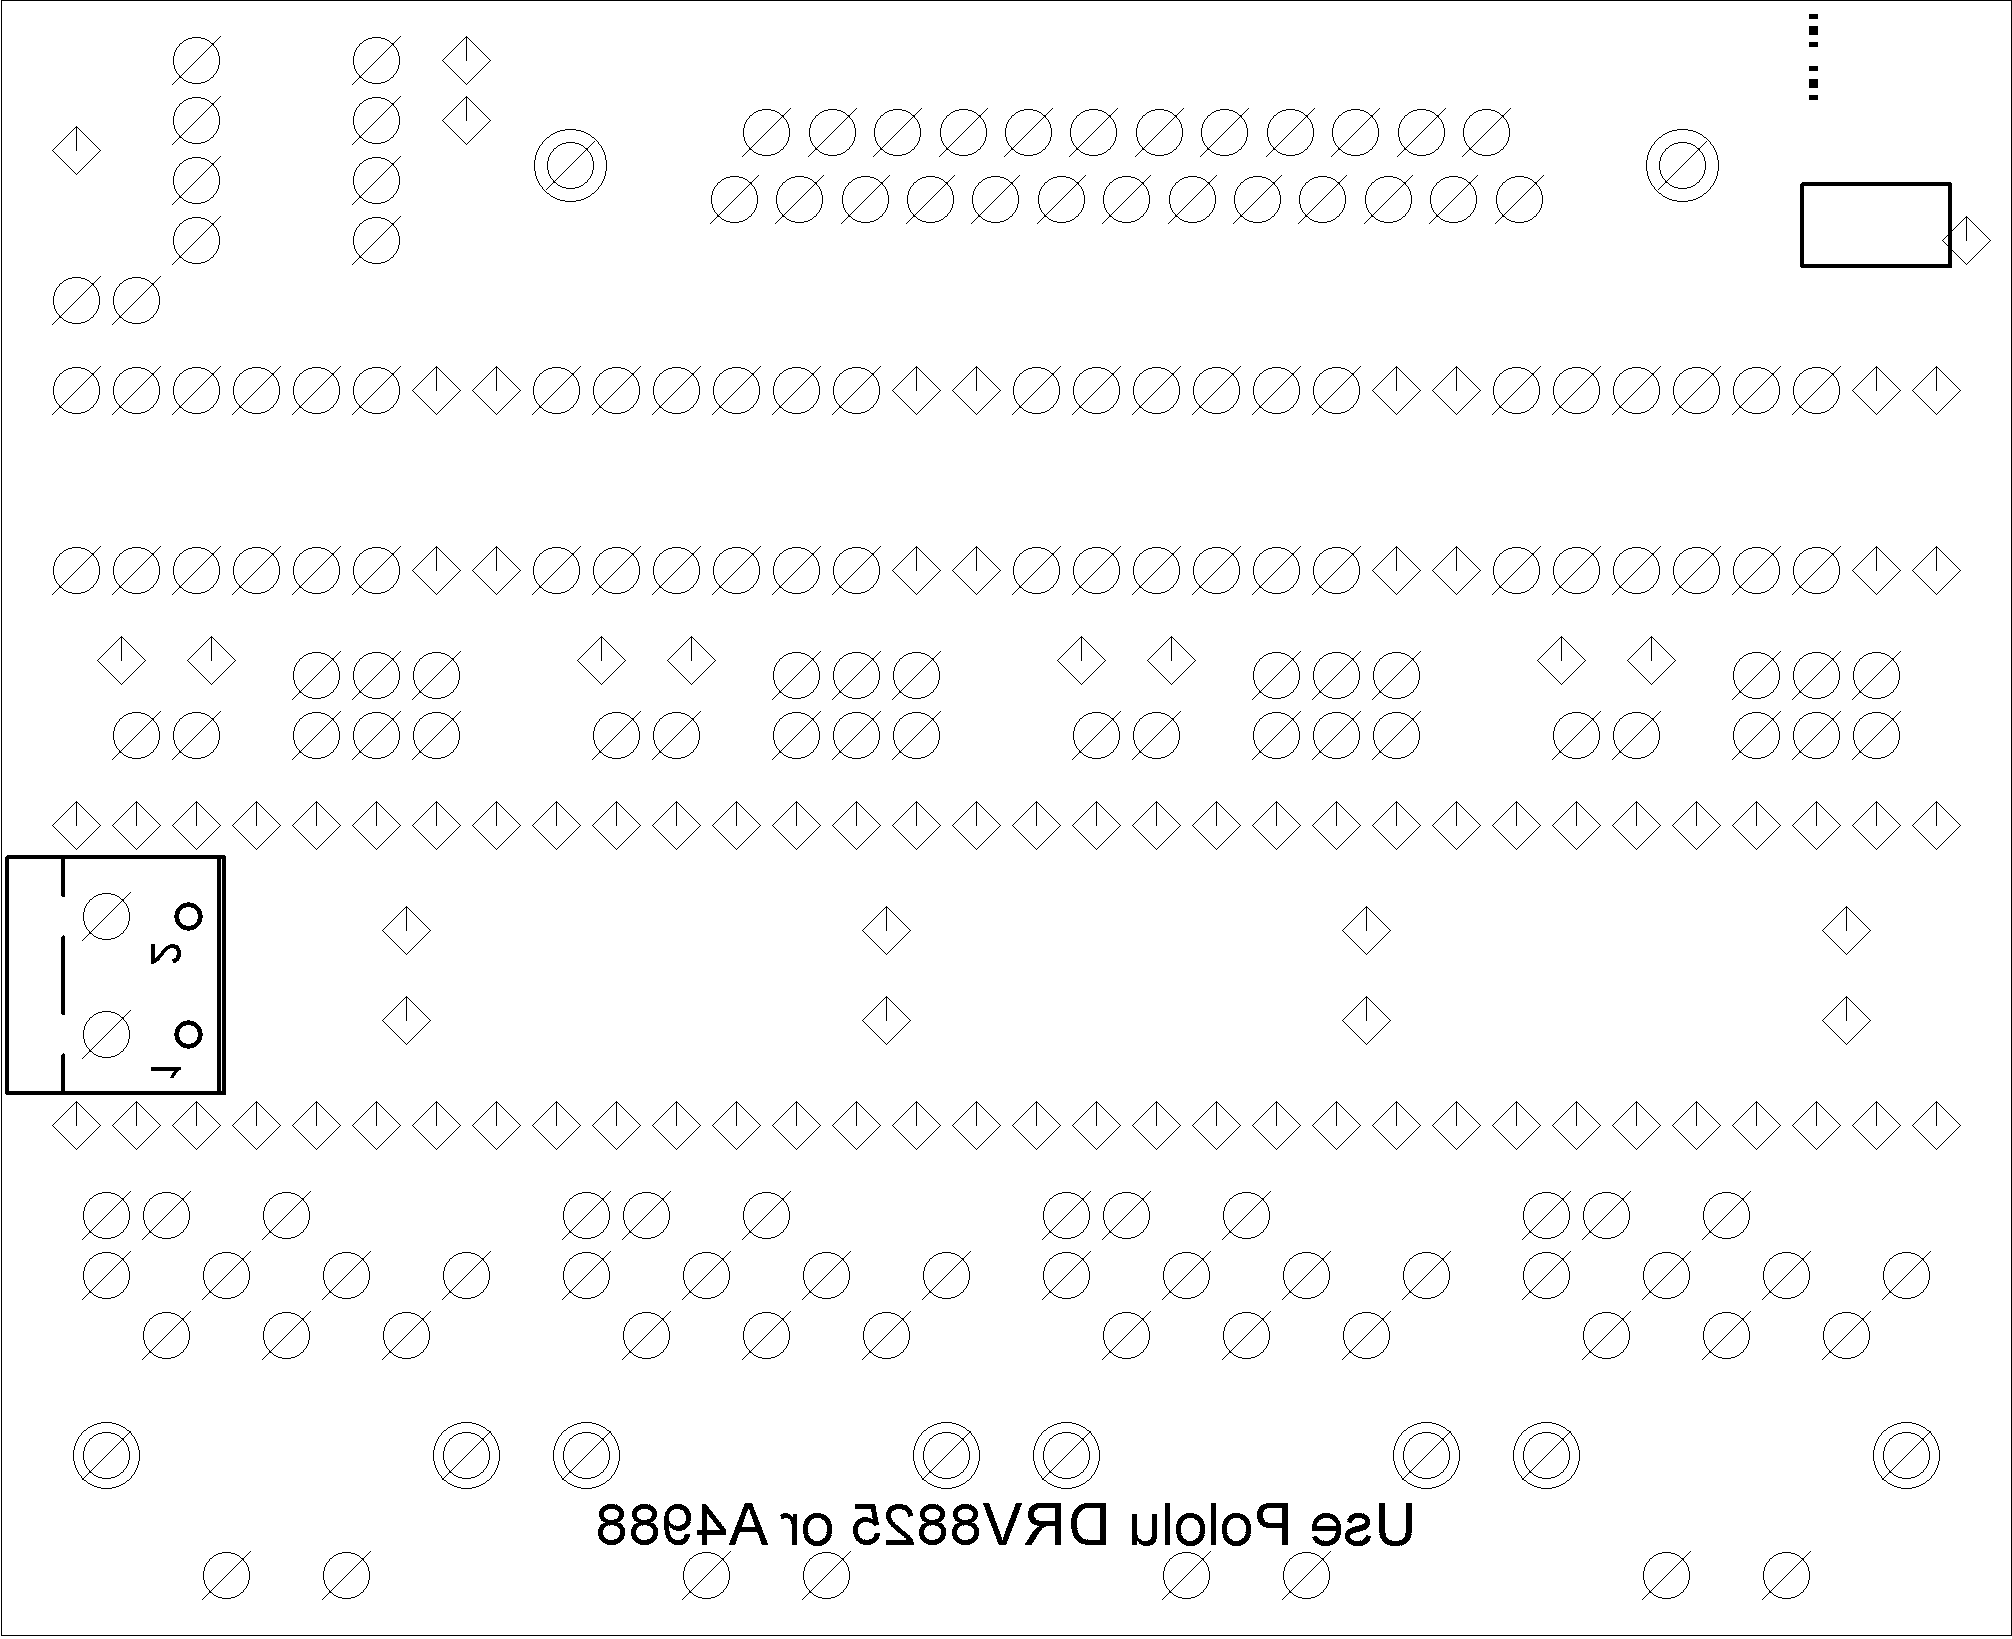
\includegraphics[width=1\textwidth]{pcb-design/bottomcream.png}
	\caption{Bottom Cream Layer}
	\label{fig:front}
\end{figure}
\begin{figure}[h]
	\centering
	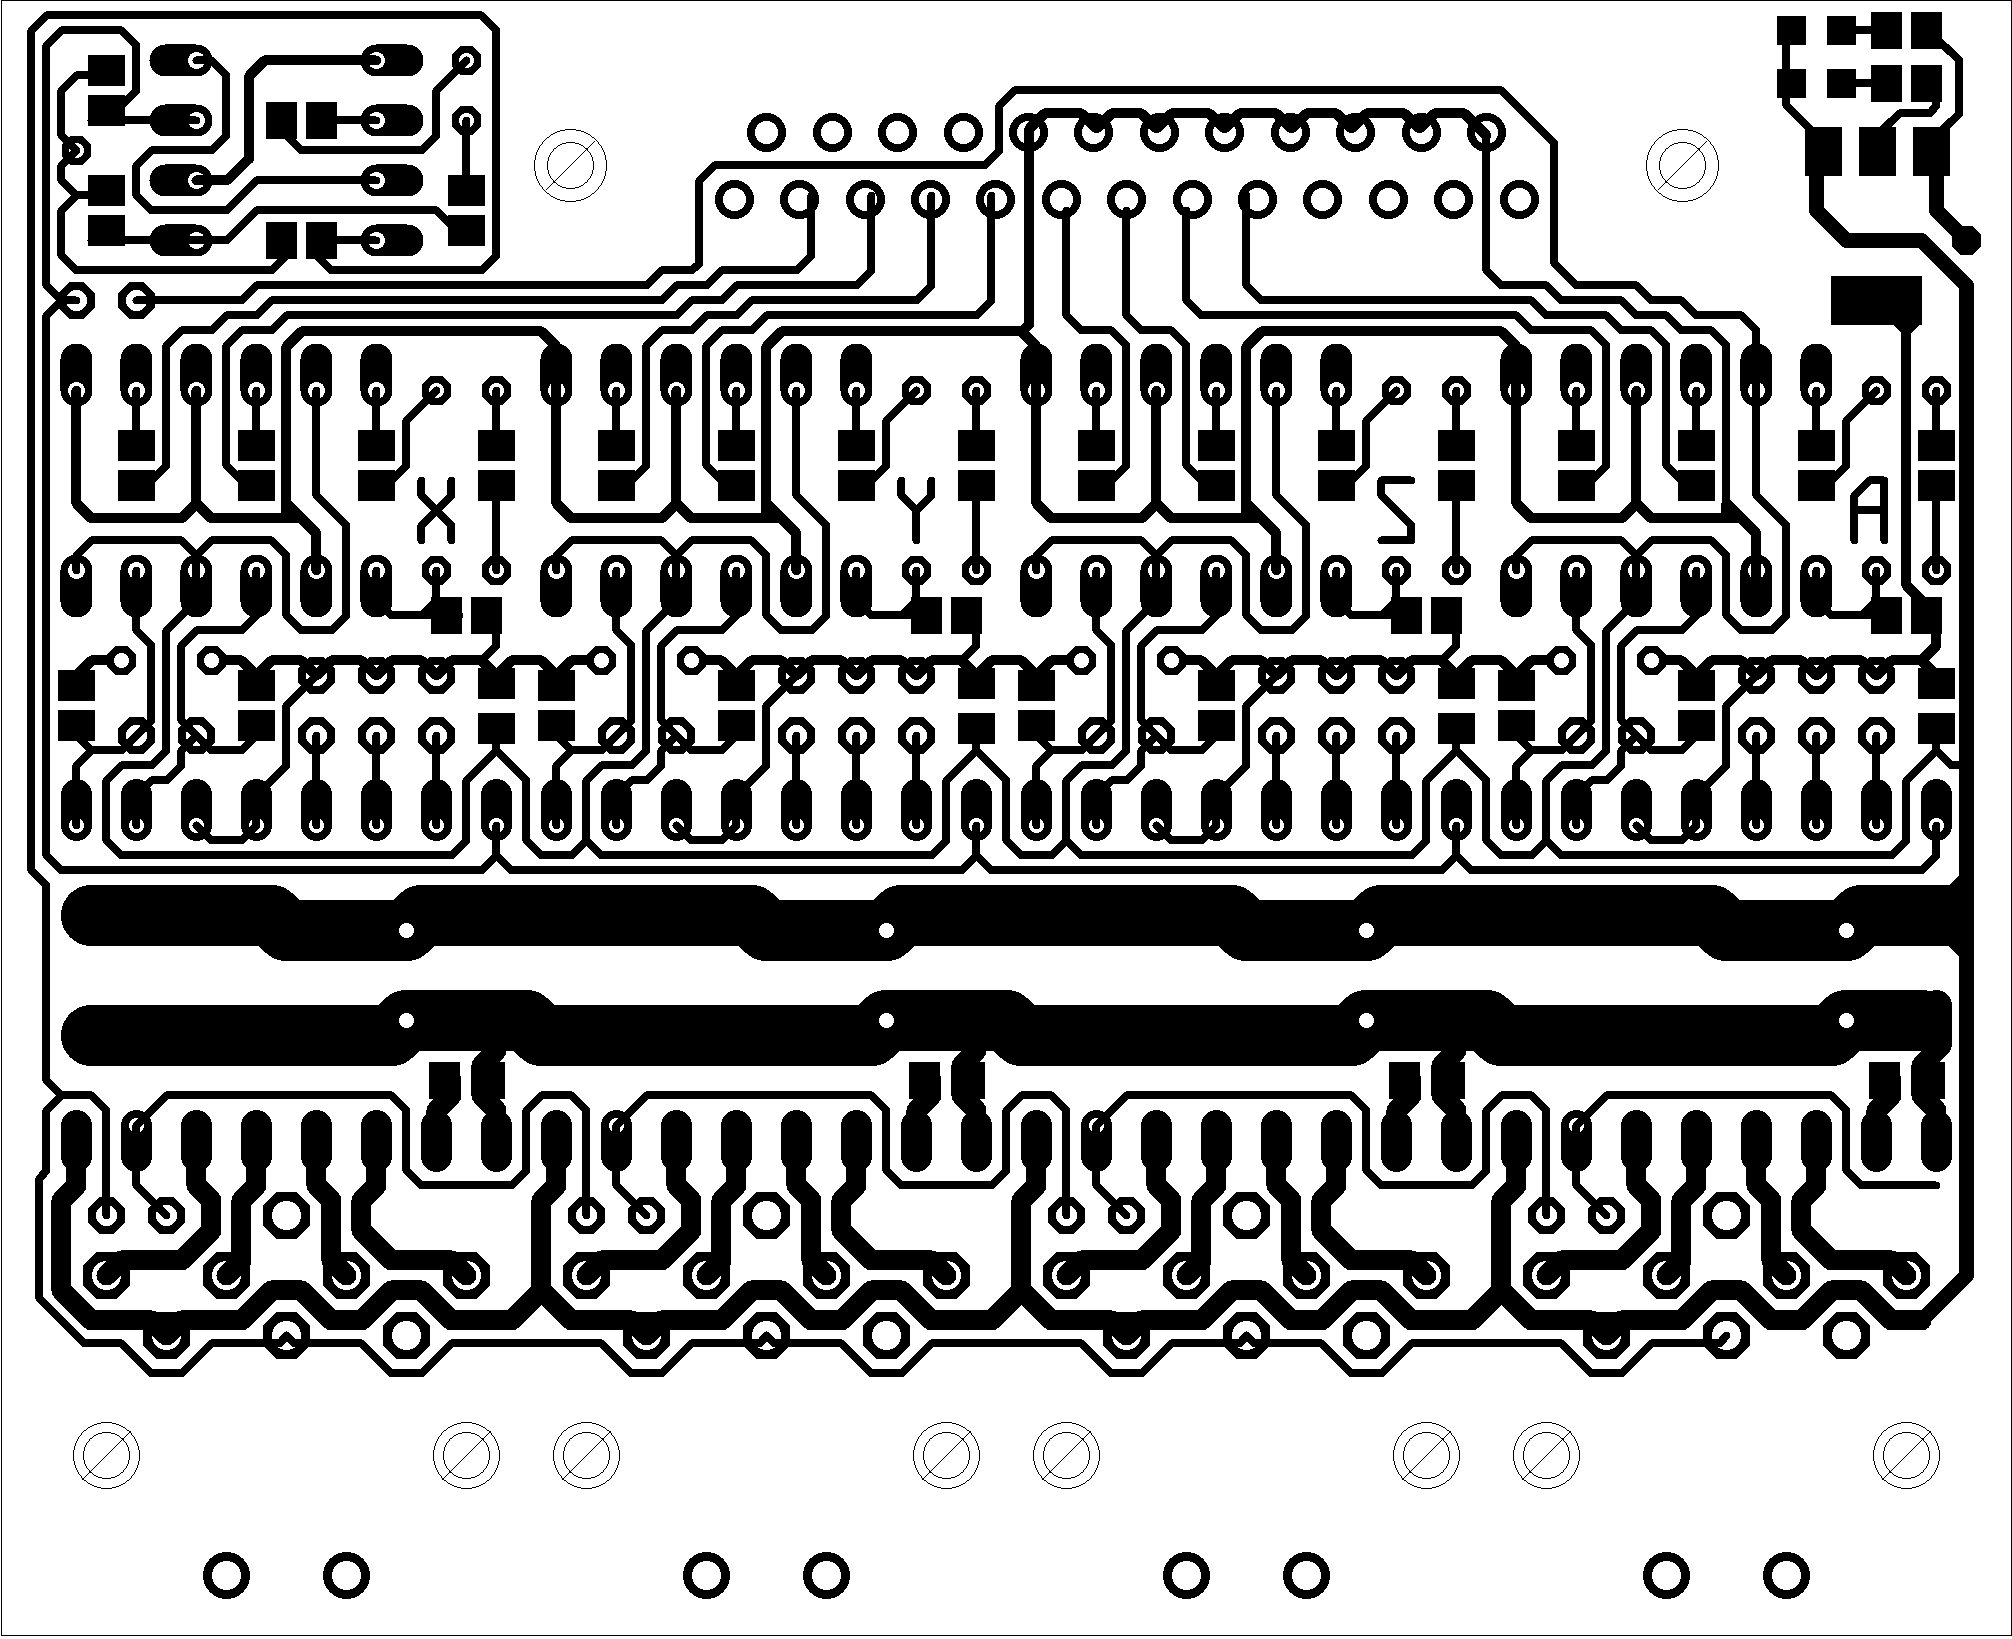
\includegraphics[width=1\textwidth]{pcb-design/bottomroute.png}
	\caption{Bottom Copper Layer}
	\label{fig:front}
\end{figure}